% ---------------------------------------------
% Alle Abbildungen 'images/' in Latex speichern 
%     * 'archiv/Pics-files.tex' 
%     * Bildgröße: 0.80/1 
% ju 06-Jun-2022 Pics-files.tex
% ---------------------------------------------
%
%\section{01_Verkaufskalkulation_Skizze}
%
%01_Verkaufskalkulation_Skizze (\autoref{fig:01_Verkaufskalkulation_Skizze}).% Referenz
%
\begin{figure}[!hb]% hier: !hb
    \centering
  \includegraphics[width=.80\textwidth]{images/01_Verkaufskalkulation_Skizze.pdf}%
  \caption{01_Verkaufskalkulation_Skizze}%\label{fig:01_Verkaufskalkulation_Skizze}%% anpassen
\end{figure}

%\newpage
%\section{02_Umsatzerloese_Skizze}
%
%02_Umsatzerloese_Skizze (\autoref{fig:02_Umsatzerloese_Skizze}).% Referenz
%
\begin{figure}[!hb]% hier: !hb
    \centering
  \includegraphics[width=.80\textwidth]{images/02_Umsatzerloese_Skizze.pdf}%
  \caption{02_Umsatzerloese_Skizze}%\label{fig:02_Umsatzerloese_Skizze}%% anpassen
\end{figure}

%\newpage
%\section{03_Kalkulationsfaktor_Skizze}
%
%03_Kalkulationsfaktor_Skizze (\autoref{fig:03_Kalkulationsfaktor_Skizze}).% Referenz
%
\begin{figure}[!hb]% hier: !hb
    \centering
  \includegraphics[width=.80\textwidth]{images/03_Kalkulationsfaktor_Skizze.pdf}%
  \caption{03_Kalkulationsfaktor_Skizze}%\label{fig:03_Kalkulationsfaktor_Skizze}%% anpassen
\end{figure}

%\newpage
%\section{Arbeitszeitermittlung}
%
%Arbeitszeitermittlung (\autoref{fig:Arbeitszeitermittlung}).% Referenz
%
\begin{figure}[!hb]% hier: !hb
    \centering
  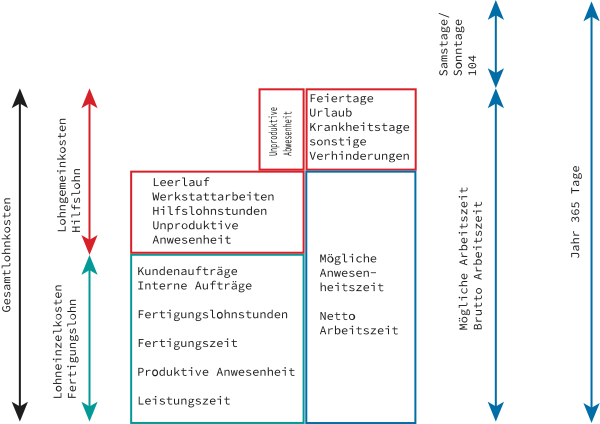
\includegraphics[width=.80\textwidth]{images/Arbeitszeitermittlung.pdf}%
  \caption{Arbeitszeitermittlung}%\label{fig:Arbeitszeitermittlung}%% anpassen
\end{figure}

%\newpage
